\section{Appendix}
\subsection{Robustness Checks}
When we compare the baseline results to results of several sample splits there are few changes to the baseline results in the expert sample. When asked about the intentions behind entering the rescue program the findings from the baseline regression persist among all sample splits. The effect in the sample of countries with high levels of unemployment becomes smaller and is only significant at the five percent level. In the sample of southern European countries the disagreement over whether lender countries wanted to impose institutional change on borrower countries also decreases and is only significant at the five percent level. Interestingly, the estimates for the sample of periphery countries are much larger than in the baseline sample. In the periphery sample participants from program countries are 19.1 percentage points less likely to agree with the statement that the lender countries wanted to help the borrowing countries and 14.2 percentage points more likely to agree that lender countries wanted to impose institutional change compared to respectively 13.1 and 11.1 percentage points in the full sample.\\
When asked about the emotions of citizens in borrower and lender countries the estimates become slightly smaller in the southern European, periphery and high debt sample than for the full sample. The divergence in assessments about whether the rescue program made the citizens in the borrower countries feel inferior even becomes insignificant in the Southern European sample. Among bot samples there is substantial disagreement between program and non-program countries that Greece will repay it's debt. 
\\
\begin{figure} [h!]
    \begin{center}
     \caption{ Intentions of the borrower countries}
    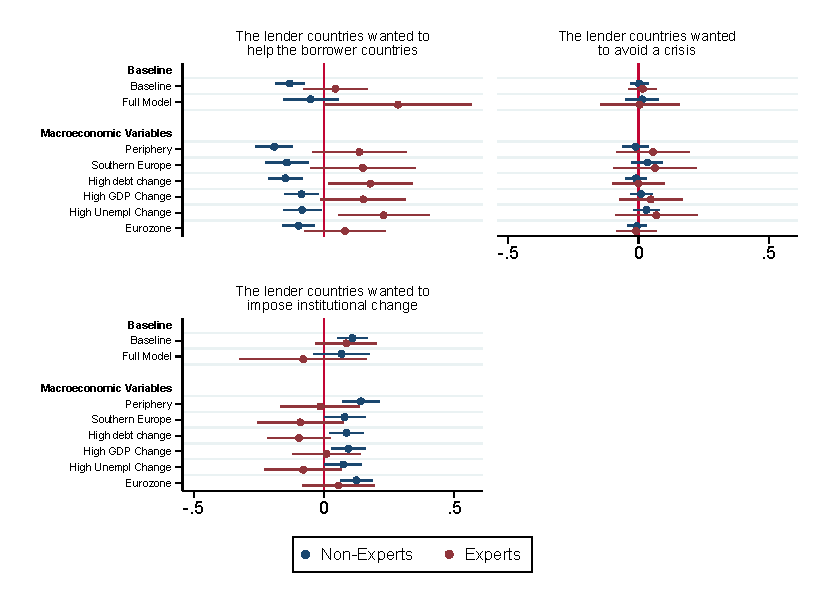
\includegraphics[scale=1.2]{Question2_samplesplits.pdf}
    \label{fig:my_label}
    \end{center}
    \tiny 
    \tablenotes{Participants were asked to assess the following statements:  Question 2.1: The lender countries wanted to help the borrowing countries Question 2.2: The lender countries wanted to help themselves avoid a crisis at home Question 2.3: The lender countries wanted to impose institutional change upon the borrower countries }
\end{figure}
\begin{figure}[h!]
    \begin{center}
     \caption{Sentiments of borrower countries (Macro Variables)}
    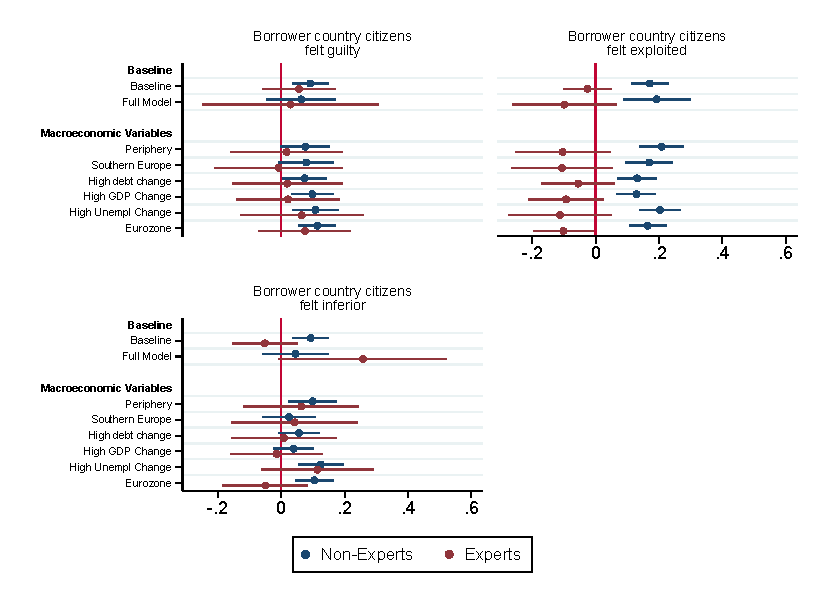
\includegraphics[scale=1.2]{Question51_samplesplits.pdf}
    \label{fig:my_label}
    \end{center}
    \tiny 
     \tablenotes{Question 5.1: The rescue experience made many citizens in the borrower countries feel guilty; Question 5.2: The rescue experience made many citizens in the borrower countries feel exploited; Question 5.3: The rescue experience made many citizens in the borrower countries feel inferior} 
\end{figure}
\begin{figure}[h!]
    \begin{center}
     \caption{Sentiments of lender countries(Macro Variables)}
    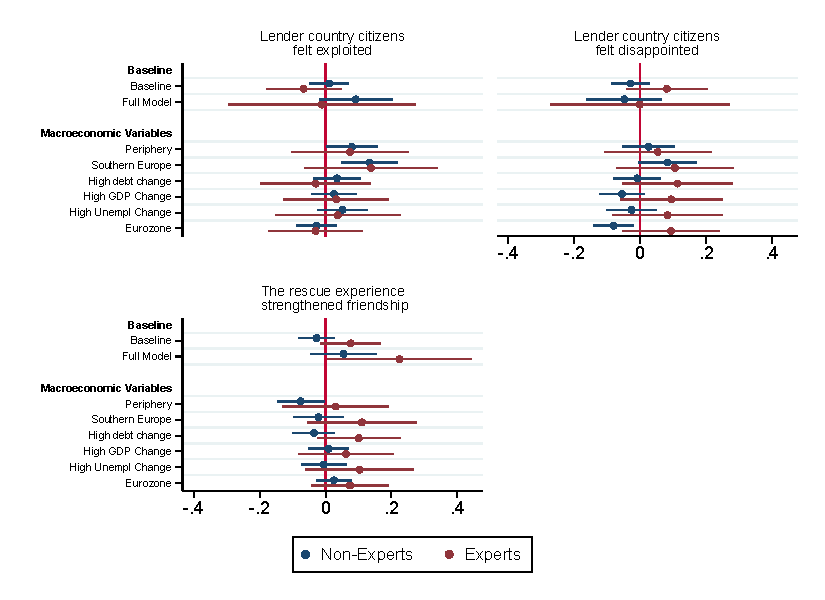
\includegraphics[scale=1.2]{Question52_samplesplits.pdf}
    \end{center}
    \tiny
     \tablenotes{Question 5.4: The rescue experience made many citizens in the lender countries feel exploited; Question 5.5 The rescue experience made many citizens in the lender countries feel disappointed Question 5.6: The rescue experience strengthened friendships between citizens Question 7: Greece will fully pay back it's debt}
\end{figure}
\begin{figure}[h!]
    \begin{center}
     \caption{Who initiated and benefited from the rescue program (Macro Variables)}
    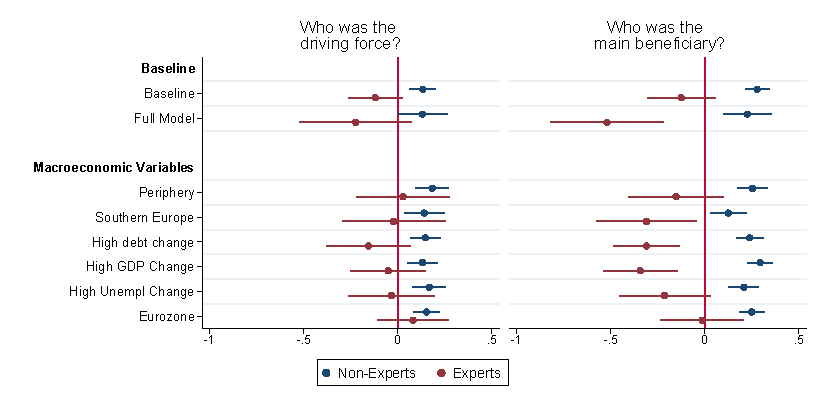
\includegraphics[scale=1.2]{macro_S_1301_S_1401.pdf}
    \end{center}
    \tiny
    \tablenotes{Question 3: Who was the driving force behind signing the memorandum; Question 4: Who was the main beneficiary of the program; }
\end{figure}
    
\begin{figure}[h!]
    \begin{center}
     \caption{Situation in Greece (Macro Variables}
    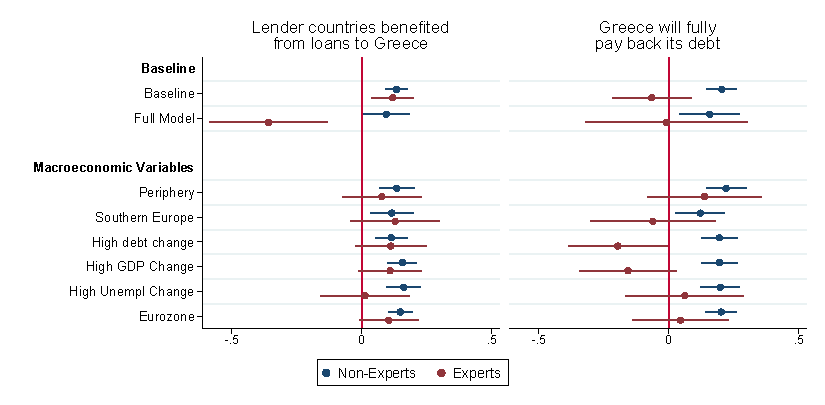
\includegraphics[scale=1.2]{macro_S_1601_S_1701.pdf}
    \end{center}
    \tiny
    \tablenotes{Question 6: Who primarily benefited from the loans to Greece; Question 7: Who primarily benefited from the loans to Greece}
\end{figure}
    \clearpage
\textbf{Ordered and Multinomial Estimation}
Participants have multiple answer possibilities. Depending on the question participants are able to rank their level of agreement on a scale of 1 to 4 or choose between the options borrower countries, lender countries or both equally. To control if differences between participants from non-program and program countries also emerge when including all answer possibilities as regression outcomes we estimate multinomial and ordered logit models. For all questions in which participants were asked to rank their level of agreement we estimate an ordered logit model, for questions in which participants were asked to name the responsible party we estimate an multinomial logit model. The significance level in the non-expert sample remains at the same level for all but one question. For the question which party was the driving force behind the referendum the significance level changes from 0.01 percent to 0.05 percent. In the expert sample all results remain insignificant. For the question if Greece will repay it's debt the divergence in effects is only significant at the 5 percent level and no longer the 1 percent level. In the majority of cases the the magnitude of effects is the same for different answer possibilities. This suggests that differences between program and non-program countries exist across all answer possibilities. \\

\\
\textbf{Inattentive Respondents}
Since we distributed our survey for the non-expert sample online we will also control for the influence of inattentive respondents in the non-expert sample. When distributing the survey online we already included an attention check when asking participants about socioeconomic characteristics. All participants failing this attention check were excluded from the survey. Further, we exclude all participants at the top 10 $\%$ and bottom 10 $\%$ of the survey time distribution. Excluding these participants does not change the inferences of our baseline estimation in the non-expert sample.\\


\\
\textbf{Clustered Robust Standard Errors} 
We cluster standard errors on the country level. Since we only collected data from 24 countries we adjust for the small number of clusters using the wild bootstrap method for logit regressions as suggested by \cite{cameron}.\footnote{We use the Stata command developed by \cite{roodman}} Inferences change for some questions when applying this method. Question 2.c becomes insignificant, questions 5a and 5c loose some significance and become significant at the 5 respectively 10 percent level.  \\

\textbf{Multiple Hypothesis Testing}
We also control for multiple hypothesis testing by adjusting our p-values using the Bonferroni Method. We adjust p-values by the number of questions we ask our participants. The Bonferroni correction does not change the significance level of our results. 

\end{figure}

\subsection{Heterogeneity Analysis}
\textbf{Socioeconomic Characteristics}
 Experts and non-experts differ along various dimensions such as education, age and gender.
 According to \cite{baumeister} events experienced at a younger age might have a more defining impact. Since the European debt crisis was accompanied for example by a high level of youth unemployment it might seem plausible that the divergences in memory might be more pronounced among the younger generation. Thus, we estimate the effect of belonging to a program country among participants older than 35 among the sample of non-experts.  The effect of the program variable on the likelihood to agree that the lender countries wanted to impose institutional change or that the rescue experience made citizens in the borrower countries feel guilty is smaller and the significance level decreases to 5 percent. For the remaining questions the overall magnitude and significance level of the program effect stays the same. 
\\
The level of education of participants may well influence the estimates. Participants with a higher level of education might have different political attitudes or consume and access different types of media. Hence, we split the non-expert sample and estimate our model only for participants reporting to have completed tertiary education. We do not find any change in the magnitude and significance level of effects for this subsample. 
\\
One dimension along which experts and non-experts differ is their degree of mobility. Experts working in think tanks or research institutes might live or have studied abroad for some time. Due to this circumstance experts might identify less with their nation than non-experts and consequently will not have a strong nation-serving bias. Unfortunately we don't have information about whether participants in the non-expert have lived or studied abroad. However, we can identify if people reported to be living in a different country than their country of birth. This applies to 25 percent of the non-expert subsample. 20.72 percent of participants from program countries and 25.45 percent from non-program countries report to be living in a different country than their country of birth. Estimating our model for this subsample changes the results quite a bit. Divergence between citizens from program- and non-program countries remains in the assessment if lender countries wanted to help borrowing countries and if the rescue experience made the citizens in the borrower countries feel exploited. For the other questions the difference in answers between program- and non-program countries becomes smaller and even vanishes completely for some questions. Hence, it appears that a higher level of mobility might be causal for the differential effects between expert and non-expert sample.  \\
\begin{figure} [h!]
    \begin{center}
     \caption{ Intentions of the borrower countries}
    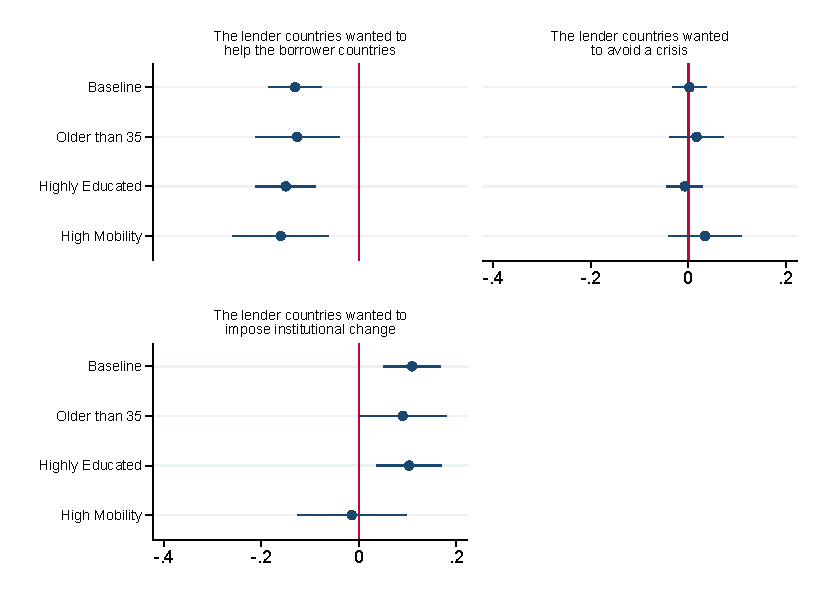
\includegraphics[scale=1.2]{socio_question2.pdf}
    \label{fig:my_label}
    \end{center}
    \tiny 
    \tablenotes{Participants were asked to assess the following statements:  Question 2.1: The lender countries wanted to help the borrowing countries Question 2.2: The lender countries wanted to help themselves avoid a crisis at home Question 2.3: The lender countries wanted to impose institutional change upon the borrower countries }
\end{figure}
\begin{figure}[h!]
    \begin{center}
     \caption{ Emotions of program countries}
    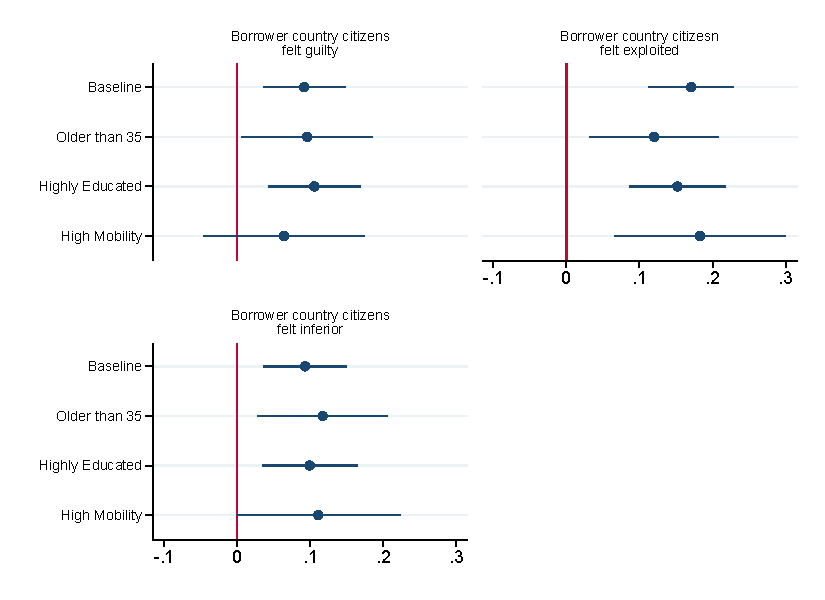
\includegraphics[scale=1.2]{socio_question5_1.pdf}
    \label{fig:my_label}
    \end{center}
    \tiny 
     \tablenotes{Question 5.1: The rescue experience made many citizens in the borrower countries feel guilty; Question 5.2: The rescue experience made many citizens in the borrower countries feel exploited; Question 5.3: The rescue experience made many citizens in the borrower countries feel inferior} 
\end{figure}
\begin{figure}[h!]
    \begin{center}
     \caption{ Emotions of non-program countries and repayment of outstanding debt}
    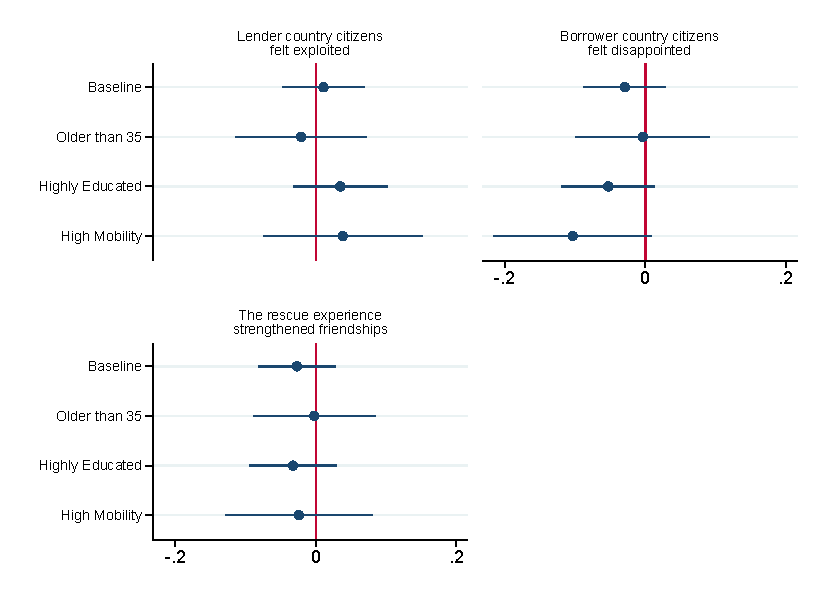
\includegraphics[scale=1.2]{socio_question5_2.pdf}
    \end{center}
    \tiny
     \tablenotes{Question 5.4: The rescue experience made many citizens in the lender countries feel exploited; Question 5.5 The rescue experience made many citizens in the lender countries feel disappointed Question 5.6: The rescue experience strengthened friendships between citizens Question 7: Greece will fully pay back it's debt}
\end{figure}
\begin{figure}[h!]
    \begin{center}
     \caption{Who initiated and benefited from the rescue program}
    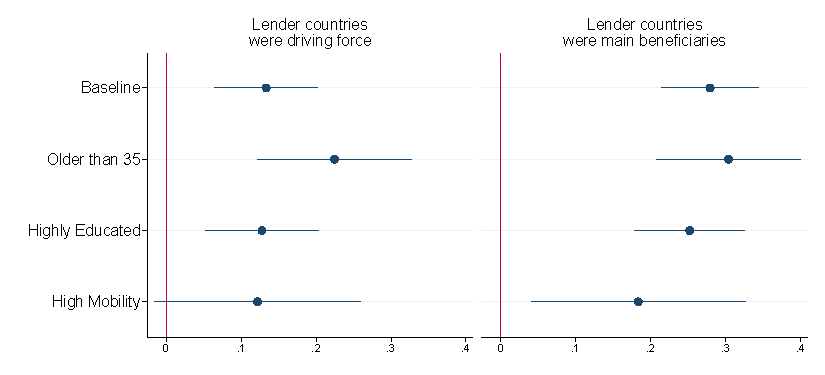
\includegraphics[scale=1.2]{socio_question3_4.pdf}
    \end{center}
    \tiny
    \tablenotes{Question 3: Who was the driving force behind signing the memorandum; Question 4: Who was the main beneficiary of the program; Question 7: Who primarily benefited from the loans to Greece}
\end{figure}
\begin{figure}[h!]
    \begin{center}
     \caption{Situation in Greece}
    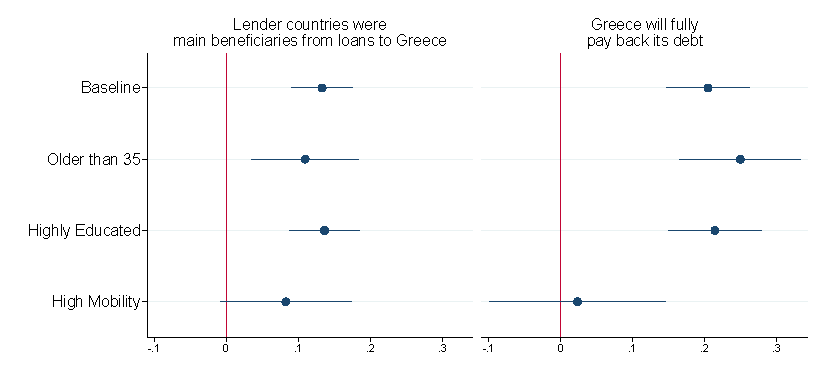
\includegraphics[scale=1.2]{socio_question6_7.pdf}
    \end{center}
    \tiny
    \tablenotes{Question 6: Who primarily benefited from the loans to Greece? ;  Question 7: Greece will fully pay back it's debt}
\end{figure}
\clearpage


\textbf{Knowledge and Beliefs}
Participants differ in their level of knowledge about the European debt crisis. Some people fail to correctly identify their country as a borrower or lender country. An overview of the fraction of participants who knew their country's status can be found in the appendix. However, knowledge about the status of one's country does not appear to influence the observed effects. The estimates of the baseline model on the subsample of non-experts who could correctly identify their country does not change in comparison to the estimates for the full sample. 

\\\\
We redefine the program variable according to the beliefs of the survey participants. We now estimate the divergence in answers between participants which believed to be the national of a  lender country and participants which believed to be the national of a borrower country. Replacing the program variable by beliefs about belonging to a program country yields different results than the baseline model. In comparison to participants who believe to be lenders, participants who believe to be borrowers do not agree less that lender countries wanted to help borrower countries. They also do not agree more that the rescue program made citizens in the borrower countries feel guilty or inferior and or less likely to state that the lender countries were the driving force behind signing the referendum. Interestingly, differences emerge in the agreement about the feelings of citizens in the lender countries. Participants who believe they live in borrower countries are less likely to agree that citizens in the lender countries felt exploited or disappointed. They are further more likely to believe that the rescue program strengthened friendships between citizens. \\

\\
Our heterogeneity analysis yields some interesting observations about potential drivers of the observed differences between expert and non-expert sample. The comparison of means suggests that the observed differences are not driven by the opinion of experts resembling the opinion of non-experts from either program or non-program countries. 
Our analysis suggests that the observed difference between experts and non-experts cannot be explained by differential effects across age or education levels. However, it appears that non-experts which are more mobile do not show a strong nation-serving bias in their assessments of the European debt crisis. Interestingly, being able to correctly identify one's country as a program or a lender country does not change the observed magnitude of results. The magnitude of effects does change however, when redefining the program variable according to beliefs of people. This suggests that collective memory might work on a more subconscious level regardless of the level of information participants have. 
\\
\begin{figure} [h!]
    \begin{center}
     \caption{ Intentions of the borrower countries (Beliefs)}
    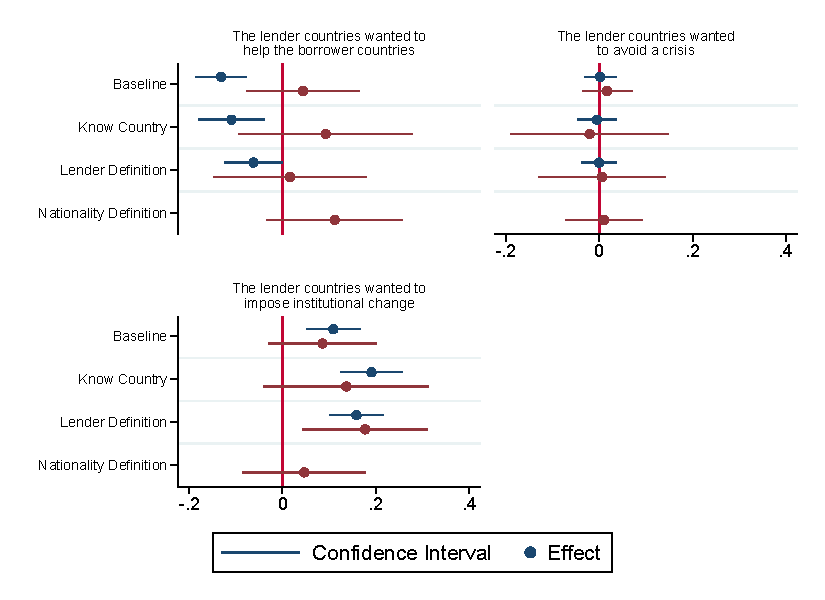
\includegraphics[scale=1.2]{belief_question2.pdf}
    \label{fig:my_label}
    \end{center}
    \tiny 
    \tablenotes{Participants were asked to assess the following statements:  Question 2.1: The lender countries wanted to help the borrowing countries Question 2.2: The lender countries wanted to help themselves avoid a crisis at home Question 2.3: The lender countries wanted to impose institutional change upon the borrower countries }
\end{figure}
\begin{figure}[h!]
    \begin{center}
     \caption{ Emotions of program countries (Beliefs) }
    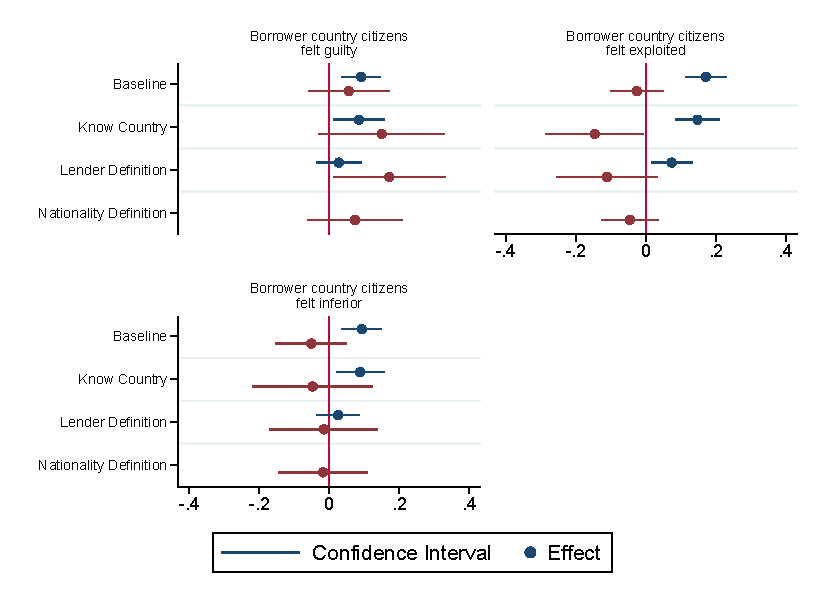
\includegraphics[scale=1.2]{belief_question51.pdf}
    \label{fig:my_label}
    \end{center}
    \tiny 
     \tablenotes{Question 5.1: The rescue experience made many citizens in the borrower countries feel guilty; Question 5.2: The rescue experience made many citizens in the borrower countries feel exploited; Question 5.3: The rescue experience made many citizens in the borrower countries feel inferior} 
\end{figure}
\begin{figure}[h!]
    \begin{center}
     \caption{ Emotions of non-program countries and repayment of outstanding debt (Beliefs)}
    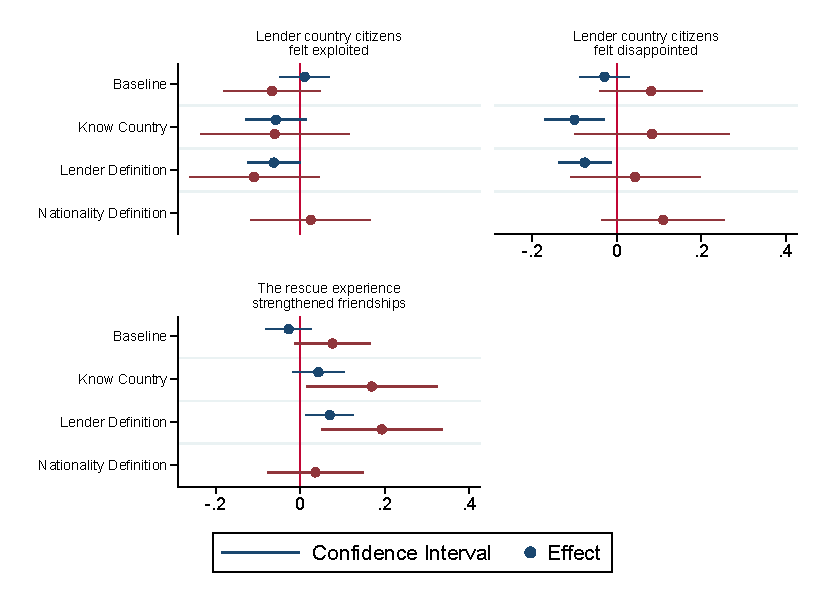
\includegraphics[scale=1.2]{belief_question52.pdf}
    \end{center}
    \tiny
     \tablenotes{Question 5.4: The rescue experience made many citizens in the lender countries feel exploited; Question 5.5 The rescue experience made many citizens in the lender countries feel disappointed Question 5.6: The rescue experience strengthened friendships between citizens Question 7: Greece will fully pay back it's debt}
\end{figure}
\begin{figure}[h!]
    \begin{center}
     \caption{Who initiated and benefited from the rescue program (Beliefs) }
    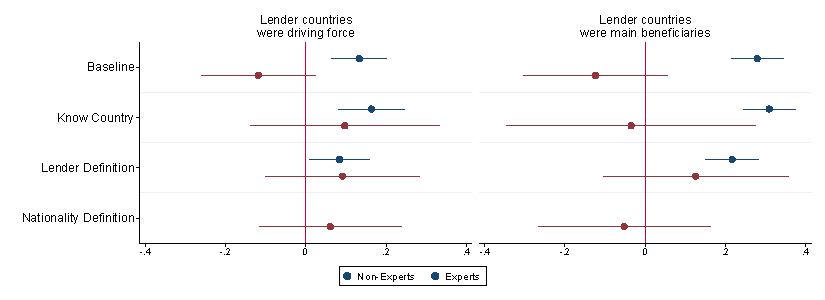
\includegraphics[scale=1.2]{belief_question34.pdf}
    \end{center}
    \tiny
    \tablenotes{Question 3: Who was the driving force behind signing the memorandum; Question 4: Who was the main beneficiary of the program; Question 7: Who primarily benefited from the loans to Greece}
\end{figure}
\begin{figure}[h!]
    \begin{center}
     \caption{Situation in Greece (Beliefs)}
    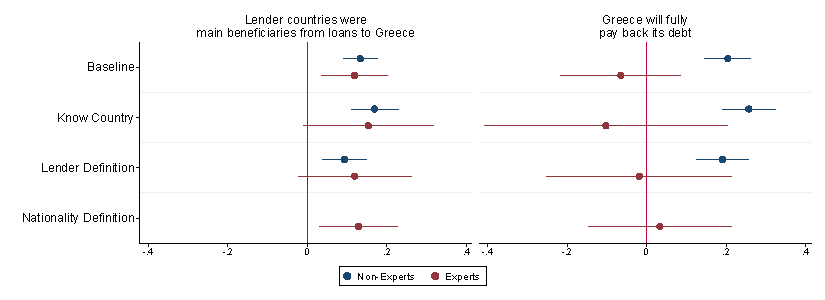
\includegraphics[scale=1.2]{belief_question67.pdf}
    \end{center}
    \tiny
    \tablenotes{Question 6: Who primarily benefited from the loans to Greece? ;  Question 7: Greece will fully pay back it's debt}
\end{figure}










